\begin{center}
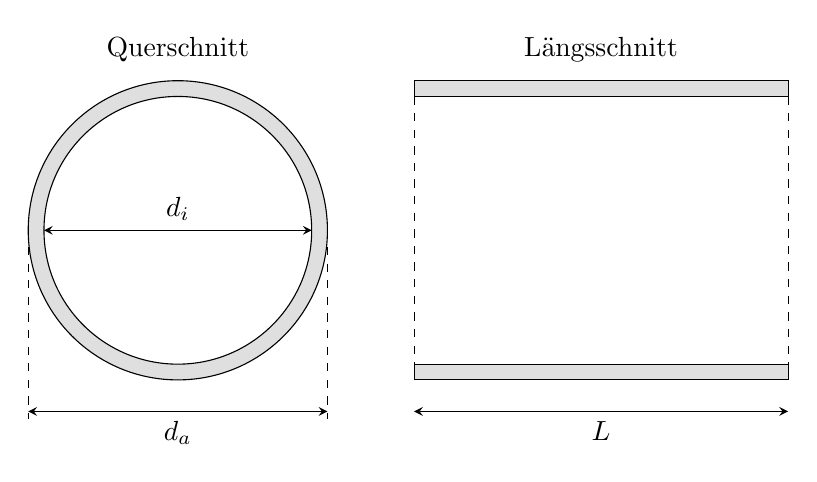
\begin{tikzpicture}[>=stealth]
 \fill[gray!25, even odd rule] (0,0) circle (1.9) (0,0) circle (1.7);
 \draw (0,0) circle (1.9) (0,0) circle (1.7);
 \draw[<->] (-1.7,0) -- (1.7,0) node[midway, above] {$d_\text{i}$};
 \draw[dashed] (-1.9,0) -- (-1.9,-2.4) (1.9,0) -- (1.9,-2.4);
 \draw[<->] (-1.9,-2.3) -- (1.9,-2.3) node[midway, below] {$d_\text{a}$};
 \node at (0,2.3) {Querschnitt};
 \fill[gray!25] (3,1.7) rectangle (7.75,1.9) (3,-1.9) rectangle (7.75,-1.7);
 \draw (3,1.7) rectangle (7.75,1.9) (3,-1.9) rectangle (7.75,-1.7);
 \draw[dashed] (3,1.7) -- (3,-1.7) (7.75,1.7) -- (7.75,-1.7);
 \draw[<->] (3,-2.3) -- (7.75,-2.3) node[midway, below] {$L$};
 \node at (5.375,2.3) {Längsschnitt};
\end{tikzpicture}
\end{center}

Der Querschnitt der Röhre ist ein Kreisring mit der Fläche
\begin{align}
 A &= \frac{\pi}{4}\left(d_\text{a}^2-d_\text{i}^2\right)
\end{align}
Das Volumen $V = A\,L$ folgt aus der Masse und der Dichte von Beton, $\rho = \rBeO$ (FoTaBe S.~187): $V = m/\rho$. Also ist
\begin{align}
 L &= \frac{m}{\rho\,A} = \LRF \\
   &= \frac{4\cdot\mBe}{\rBe\cdot\pi\cdot\left(\left(\dAu\right)^2-\left(\dIn\right)^2\right)} \\
   &= \LR \approx \result{\LRP{0}{2}}
\end{align}
